\section{Evaluación}
\label{sec:estudiorend}

En esta sección describiremos las aplicaciones descritas para evaluar la integración \textit{COMPSs+OmpSs-2}, los entornos donde haremos la evaluación y los resultados de esta.  

\subsection{Aplicaciones}
\subsubsection{K-Means}

\textit{K-Means} es un algoritmo utilizado para hacer \textit{clustering} sobre un grupo de datos, es decir, agrupar los datos en \textit{clusters}. Cada dato pertenece al \textit{cluster} cuyo centro está en la distancia mínima, si no fuera así pertenecería a otro \textit{cluster}. Se inicializan \textit{clusters} con centros escogidos de manera aleatoria y se comparan las distancias a todos los \textit{clusters} y se determina a cual pertenece cada dato (siempre al centro más cercano), una vez hecho esto se vuelve a calcular el centro de cada \textit{cluster}, todo este proceso conforma una iteración de \textit{K-Means}, habitualmente se itera hasta que converge, esto es que la distancia entre los centros asignados en dos interaciones consecutivas de cada \textit{cluster} es cercana a 0.
\par\bigskip
Tal y como hemos desarrollado la aplicación tiene 4 tareas, que son \textit{init\_Fragment}, \textit{compute\_newCluster} (tiene una implementación en CPU y otra en GPU), \textit{merge\_newCluster}, \textit{update\_Clusters}. El siguiente grafo de dependencias muestra una ejecución de \textit{K-Means} con 5 fragmentos de 25 dimensiones con 200000 puntos cada uno, el número de \textit{clusters} a formar es 25 y se efectúa una única iteración. Para no sobrecargar este apartado se incluye en el apéndice \ref{sec:codigokmeans} la interfaz y el programa principal de la aplicación.

\begin{figure}[H]
	\centering 
	\caption{Grafo de dependencias entre tareas de K-Means.}
	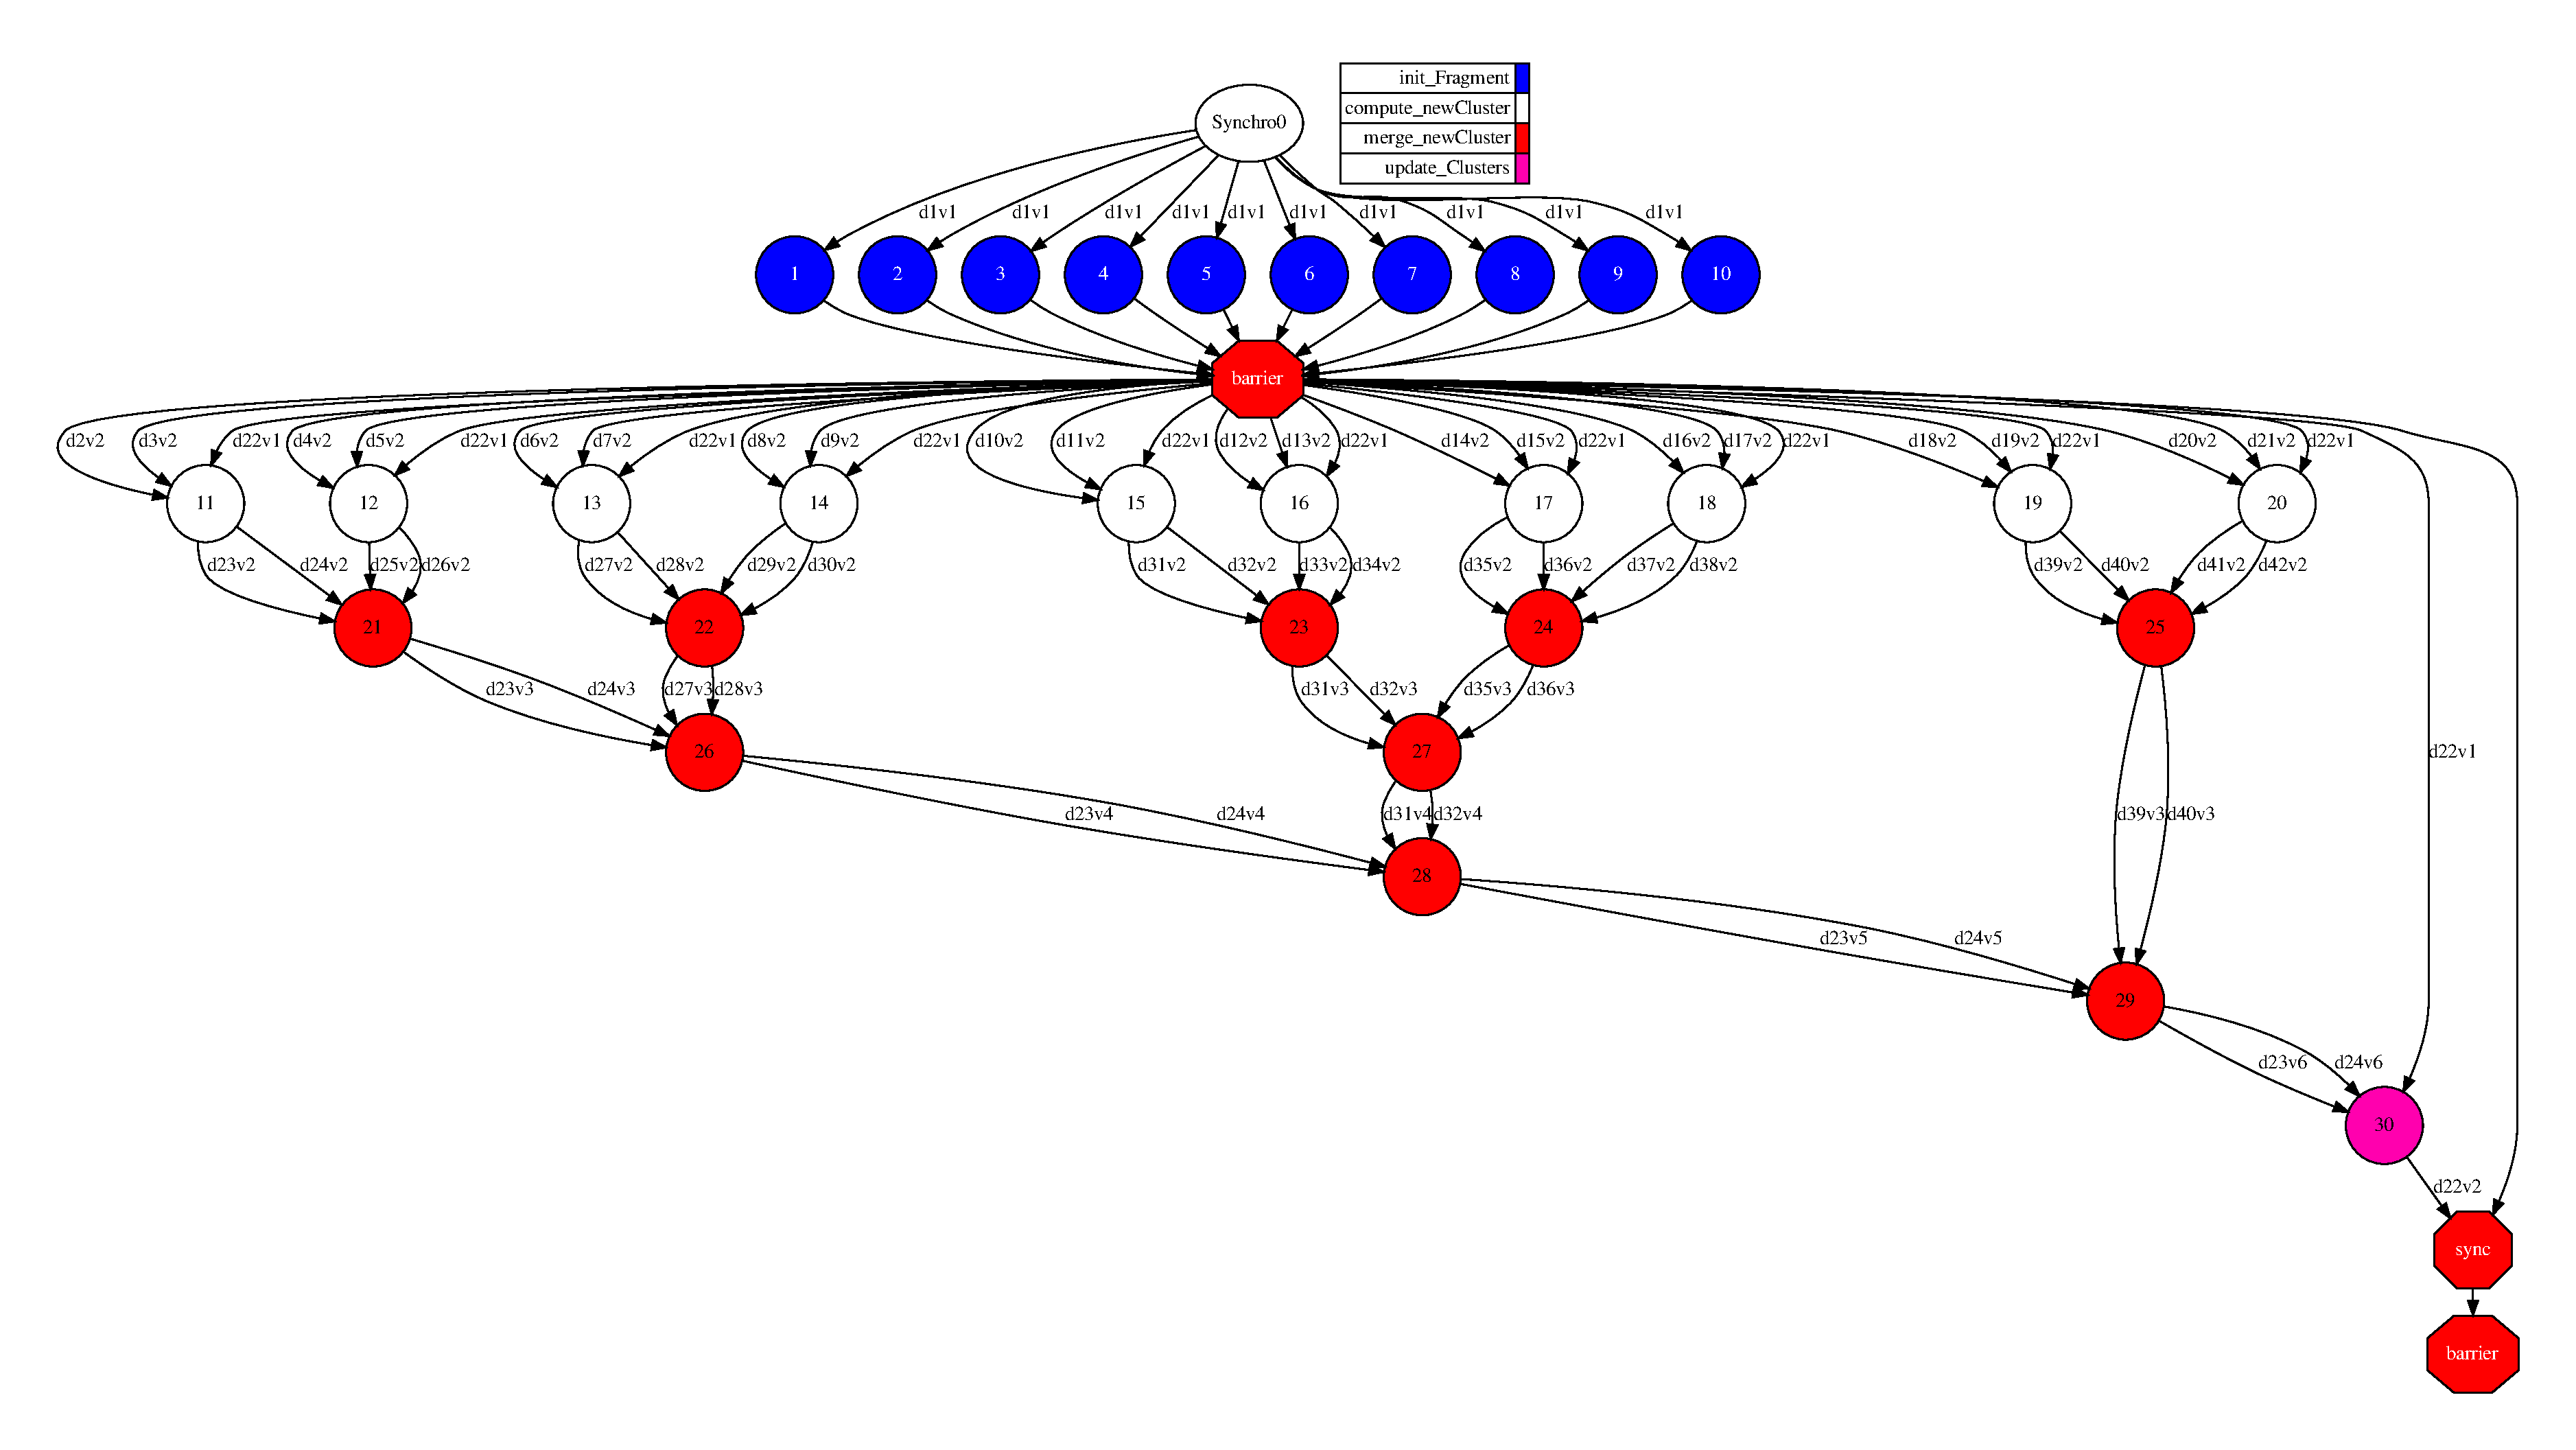
\includegraphics[scale=0.2]{grafo_kmeans.pdf}
	\label{fig:grafokmeans}
\end{figure}

\subsubsection{Cholesky}

\textit{Cholesky} es un método de descomposición aplicable cuando la matriz es simétrica definida positiva, entonces esta puede ser descompuesta como el producto de una matriz triangular inferior y su traspuesta. El método \textit{Cholesky} se utiliza para resolver sistemas de ecuaciones lineales, es similar a la descomposición \textit{LU} y es el doble de eficiente, la única restricción es que no siempre es aplicable.
\par\bigskip
La aplicación ha sido desarrollada utilizando una librería para operaciones de algebra lineal programada en \textit{C} con \textit{OmpSs} y \textit{OmpSs-2}, esta librería es \textit{LASs}\footnote{https://pm.bsc.es/mathlibs/lass} (\textit{Linear Algebra routines on OmpSs}). Las funciones que implementa \textit{LASs} serán utilizadas como tareas a nivel de \textit{COMPSs} y después una vez ejecutadas harán uso de \textit{OmpSs-2}, por lo que realmente desarrollar una aplicación utilizando una librería externa es muy sencillo.
\par\bigskip
Tiene 5 tareas, son \textit{generate\_block}, \textit{ddss\_dpotrf}, \textit{ddss\_dtrsm}, \textit{ddss\_dgemm}, \textit{ddss\_dsyrk}, la primera se utiliza para generar los bloques de manera distribuida (así el \textit{master} no tiene reservar memoria para toda la matriz, que podría ser muy grande), y las otras 4 son operaciones de algebra lineal que utilizadas de la forma correcta aplicarán el método de descomposición de \textit{Cholesky}. En el apéndice \ref{sec:codigocholesky} se encuentra la interfaz y el prorgama principal del programa.

\todo{grafo cholesky}

\subsection{Entornos para el estudio}

Para la realización del estudio del rendimiento se han utilizado dos máquinas que el \textit{Barcelona Supercomputing Center} pone a nuestra disposición, que son \textit{CTE-Power} y \textit{MareNostrum4}.

\subsubsection{CTE-Power}
\label{sec:power}

\textit{CTE-Power} es un \textit{cluster} basado en la tecnología de procesadores \textit{IBM} \textit{Power9}. Tiene 2 nodos de \textit{login}, son los nodos desde donde operan los usuarios y 52 nodos de cómputo. 
\par\smallskip
Cada nodo tiene los siguientes componentes:
\par\smallskip
\begin{itemize}
	\item 2 x \textit{IBM Power9 8335-GTH} @ 2.4GHz (3.0GHz en modo turbo), cada procesador con 20 cores cada uno con 4 \textit{threads}.
	\item 512GB de memoria organizada en 16 \textit{dimms} de 32GB @ 2666MHz.
	\item 4 x \textit{NVIDIA} V100 con 16GB \textit{HBM2}.
	\item 2 x SSD que proporcionan 1.9TB de almacenaje local.
	\item 2 x \textit{NVM Express} 3.2TB.
	\item Interfaz de red \textit{Mellanox}.
	\item Sistema de ficheros GPFS a través de fibra a 10GBit.
\end{itemize}

Nosotros utilizaremos tan sólo 10 nodos, por lo que tendremos a nuestra disposición en la mayor ejecución 1600 CPUs y 40 GPUs \textit{NVIDIA V100}. 

\subsubsection{MareNostrum4}
\label{sec:mare}

\textit{MareNostrum4} es un supercomputador basado en la tecnología de procesadores \textit{Intel Xeon Platinum} de la generación \textit{Skylake}. Tiene 5 nodos de \textit{login} y 3.456 nodos de cómputo.
\par\smallskip
Cada nodo tiene los siguientes componentes:
\par\smallskip
\begin{itemize}
	\item 2 x \textit{Intel Xeon Platinum 8160 @ 2.10GHz} con 24 cores.
	\item 96 GB de memoria organizada en 12 \textit{dimms} de 8GB @ 2667MHz.
	\item Un SSD que proporciona 200 GB de almacenaje local.
	\item 100 Gbit/s \textit{Intel Omni-Path HFI Silicon 100 Series PCI-E adapter}.
	\item 10 Gbit \textit{Ethernet}.
\end{itemize}

Igual que con \textit{CTE-Power} tan sólo utilizaremos 10  nodos, por lo tanto tendremos en la mayor ejecución 480 CPUs.

\subsection{K-Means}

La evaluación con \textit{K-Means} ha consistido en hacer un test de \textit{strong scaling}, que consiste en ejecutar la aplicación con un tamaño de problema fijo y aumentar el número de recursos de cómputo, y otro de \textit{weak scaling} donde aumentaremos de manera proporcional el tamaño del problema y los recursos de cómputo. En el apartado \ref{sec:power} describimos la máquina que utilizamos en estos test, haremos uso de todas las \textit{CPUs} y \textit{GPUs} de cada nodo.

\subsubsection{Strong scaling}

La imagen \ref{fig:sc-time} muestra una gráfica que tiene en el eje vertical el tiempo y en el horizontal el número de nodos. El tamaño del problema que se ha utilizado es de 400 fragmentos de 50 dimensiones y 200000 puntos cada uno, el número de \textit{clusters} a formar es 50 y se efectúan 5 iteraciones. Se han tomado 10 muestras de cada ejecución, la línea azul muestra la media de las muestras para el mismo número de nodos, la de color naranja muestra el tiempo ideal que debería tardar según el número de nodos. En cada punto de la línea azul se muestra la diferencia entre el máximo valor y el mínimo que se han tomado en las muestras.

\begin{figure}[H]
	\centering 
	\caption{Tiempo de ejecución al aumentar el número de recursos.}
	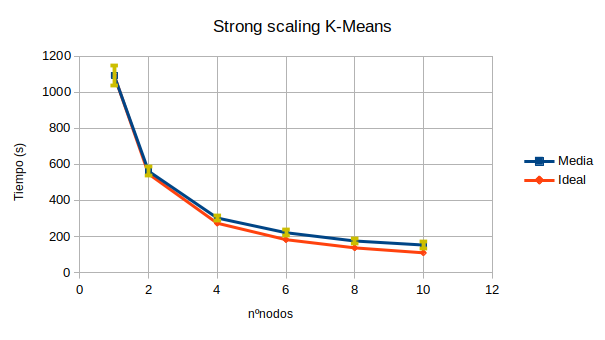
\includegraphics[scale=0.8]{estudio/KMeans/sc/kmeans-sc-time.png}
	\label{fig:sc-time}
\end{figure}

Es bueno que la línea azul sea lo más parecida a la línea naranja, eso nos indicaría que la aplicación escala perfectamente, ya que cada vez que aumentamos los recursos el tiempo de ejecución se reduciría proporcionalmente. La imagen \ref{fig:sc-speedup} muestra la misma información que \ref{fig:sc-time} dispuesta en forma de ganancia, se puede ver que se comporta bien hasta que en los 6 nodos empieza a dejar de acercarse al ideal.

\begin{figure}[H]
	\centering 
	\caption{Ganancia al aumentar el número de recursos.}
	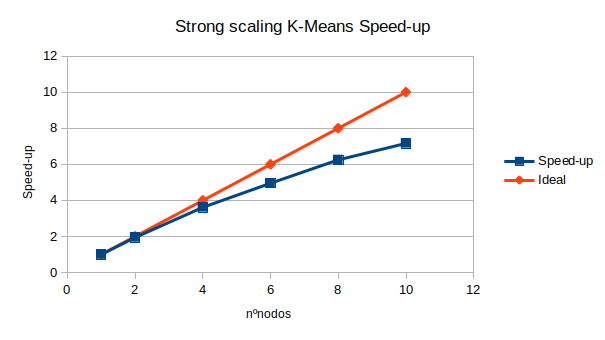
\includegraphics[scale=0.8]{estudio/KMeans/sc/kmeans-sc-speedup.png}
	\label{fig:sc-speedup}
\end{figure}

\subsubsection{Weak scaling}

En un test de \textit{weak scaling}, esperamos que los tiempos de ejecución sean siempre los mismos, ya que el tamaño del problema es siempre proporcional a los recursos de cómputo. Esto sería perfecto pero hay que efectuar comunicación entre nodos y gestionar todo el sistema, por lo que no podemos mantener este escenario ideal. La imagen \ref{fig:wc-effic} muestra cómo al aumentar el número de nodos la eficiencia baja del ideal (que el tiempo de ejecución sea siempre el mismo), pero se mantiene alrededor del mismo valor a partir de los 6 nodos.

\begin{figure}[H]
	\centering 
	\caption{Eficiencia al mantener proporcional el tamaño del problema y el número de recursos.}
	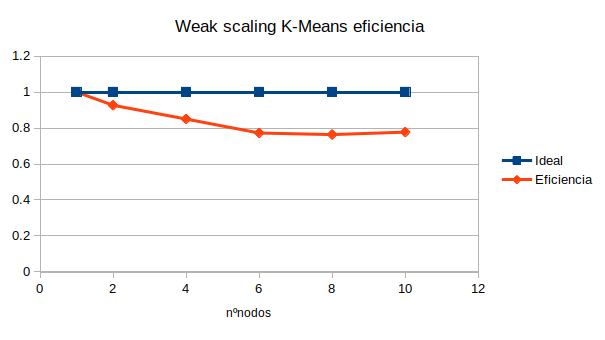
\includegraphics[scale=0.8]{estudio/KMeans/wc/kmeans-wc-efficiency.png}
	\label{fig:wc-effic}
\end{figure}

\subsection{Cholesky}







